


\chapter{Observations}
  \label{ch_rbsp}

\todo{You know what would be great for putting this numerical work in context? A nice, consistent survey that breaks down the occurrence rate of Pc4 pulsations by harmonic, etc. }

%Observations show that the poloidal mode is most excited in the second harmonic\cite{cummings_1969,hughes_1978,arthur_1981,singer_1982,takahashi_1984,engebretson_1988} even when there is a strong compressional component\cite{takahashi_1987,haerendel_1999,vaivads_2001,sibeck_2012}. 

\todo{The tools used in the present chapter --- SPEDAS and the SPICE kernel --- are publicly available. They run best with an IDL license, which is not, but they are functional using just the (free) IDL virtual machine. The code is wrapped up in a Git repository: \url{https://github.com/chizarlicious/RBSP} (maybe should make a GitHub organization to hold this code, to decouple it from my personal account?). }

Previous work:

Dai\cite{dai_2015} used RBSP to look at poloidal Pc4 events, with a bias in favor of the second harmonic --- 890 events. Events are most common near noon, but are spread across the day and dusk side, with a few stragglers at midnight. 

Anderson\cite{anderson_1990} used AMPTE/CCE (mostly $L>7$, near the equator) to look at Pc4 events --- 7000 hours. Limited commentary on parity. Toroidal modes were found to outnumber poloidal modes three-to-one. ``Harmonic toroidal resonances'' are spread 0600 to 1600. ``Fundamental toroidal resonances'' (which are not mutually exclusive with harmonic ones!) appear everywhere but dusk. 

Liu\cite{liu_2009} used THEMIS (equatorial orbit, $L$ out to \about10) to look at both poloidal and toroidal modes --- 9805 one-minute Pc4 events (?). No commentary on parity. Poloidal events are most common at noon (with another peak post-midnight) and strongest on the dusk side. Toroidal events are most common from pre-dawn to pre-noon and strongest pre-midnight and post-dawn. 

Kokubun\cite{kokubun_1989} used ATS6 (synchronous orbit) --- \about150 events. No commentary on harmonic. Toroidal events dominate in the dawn sector. Poloidal events are spread across all MLT, with a peak in the early afternoon and Pgs in the early morning. 

Motoba\cite{motoba_2015} used GOES13 and GOES15 (geosynchronous) to look specifically at Pgs --- 105 events. Seen from midnight to noon, with a strong peak before dawn, 0300 or so. 

% -----------------------------------------------------------------------------
% -----------------------------------------------------------------------------
% -----------------------------------------------------------------------------
\section{Sampling Bias and Event Selection}
  \label{sec_selection}

The present analysis makes use of all available Van Allen Probe data, which spans from October 2012 to August 2015. Between the two probes, that's just over 2000 days of observation. 

For the purposes of Pc4 pulsations, it's reasonable to consider the two probes to be independent observers. Nearly all Pc4 events occur near apogee ($L\gtrsim5$), at which point the two probes are several hours apart in MLT. Pc4 events are typically not large enough to be seen by both probes simultaneously, and not long enough in duration to be seen by two probes passing through the same region of space several hours apart. 

\todo{Quantify how often an event is seen by both probes? }

Electric and magnetic field waveforms are collected using the probes' \todo{$\cdots$} instrument. Values are cleaned up by averaging over the ten-second spin period. Three-dimensional electric field data is then obtained using the $\vec{E} \cdot \vec{B} = 0$ assumption. Notably, this assumption is taken only when the probe's spin plane is offset from the magnetic field by at least \SI{15}{\degree}. The rest of the data --- about half --- is discarded, which introduces a sampling bias against the flanks. 

A further bias is introduced by the probes' non-integer number of precessions around Earth. As of July 2014, apogee had precessed once around Earth\cite{dai_2015}. The present work considers roughly one and a half precessions; the nightside has been sampled at apogee twice as often as the dayside. 

The spatial distribution of usable data --- that is, data for which three-dimensional electric and magnetic fields are available --- is shown in \cref{fig_pos_all_sharp}. Bins are unitary in $L$ and in MLT. Event distribution in magnetic latitude is not shown; the Van Allen Probes are localized to within \about\SI{10}{\degree} of the equatorial plane. 

\todo{$L$ is italicized and MLT is not? That seems weird. }

\begin{figure}[!htb]
    \centering
    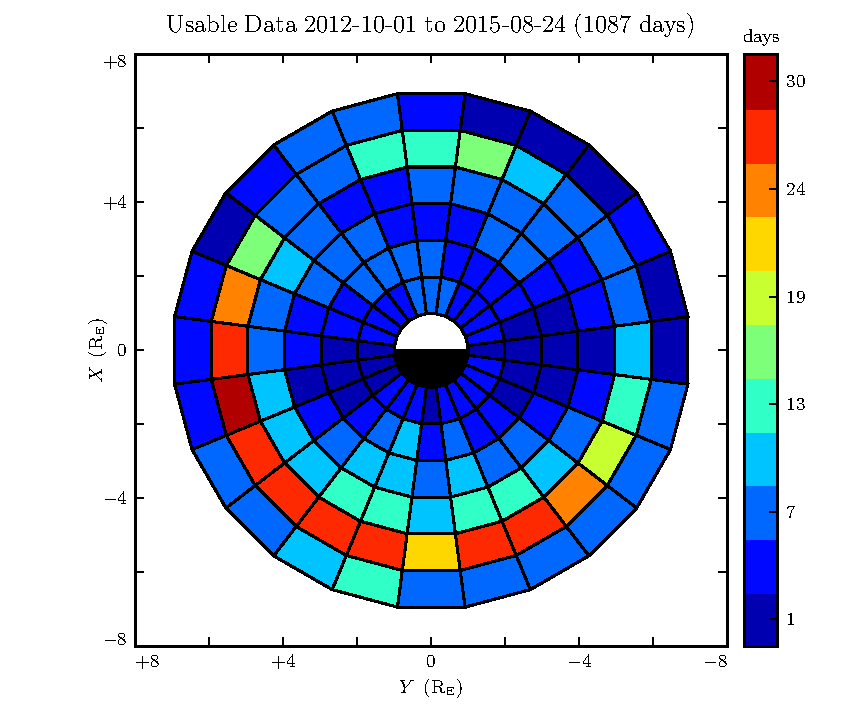
\includegraphics[width=\textwidth]{figures/pos_all_sharp.pdf}
    \caption[Distribution of Usable Van Allen Probe Data]{
      Three-dimensional electric field values are computed by assuming $\vec{E} \cdot \vec{B} = 0$. Data is discarded whenever the magnetic field falls within \SI{15}{\degree} of the spin plane, which introduces a bias against the flanks. Furthermore, the probes have completed one and a half precessions around Earth; the dayside has been sampled once at apogee, and the nightside twice. 
    }
    \label{fig_pos_all_sharp}
\end{figure}

Field measurements are transformed from GSE coordinates into the same dipole coordinates used in \cref{ch_model,ch_results}. The \z axis is parallel to the background magnetic field, which is estimated using a ten-minute running average of the magnetic field measurements. The \y axis is defined per $\yhat \parallel \zhat \times \vec{r}$. The \x axis is then defined per $\xhat \equiv \yhat \times \zhat$. This scheme guarantees that the axes are right-handed and pairwise orthogonal\cite{liu_2009}. 

The \about1000 days of usable data are considered half an hour at a time, which gives a frequency resolution of \about\SI{0.5}{\mHz} in the discrete Fourier transform. Spectra are computed for all six field components: \dft{B_x}, \dft{B_y}, \dft{B_z}, \dft{E_x}, \dft{E_y}, and \dft{E_z}. The background magnetic field is subtracted before transforming the magnetic field components, leaving only the perturbation along each axis\footnote{As in \cref{ch_model,ch_results}, $B_x$ refers not to the full magnetic field in the \x direction, but to the perturbation in the \x direction from the zeroth-order magnetic field.}. Each waveform is also shifted horizontally so that its mean over the thirty minute event is zero. 

Frequency-domain Poynting flux is computed from the electric and magnetic field transforms. A factor of $L^3$ compensates the compression of the flux tube, so that the resulting values are effective at the ionosphere. Poloidal and toroidal Poynting flux, respectively, are given by:
\begin{align}
  \dft{S_P} &\equiv -\frac{L^3}{\mz} \dft{E_y} \dft{B_x^*} &
  \dft{S_T} &\equiv  \frac{L^3}{\mz} \dft{E_x} \dft{B_y^*}
\end{align}

The poloidal and toroidal channels are independently checked for Pc4 waves. For each channel, a Gaussian profile is fit to the magnitude of the Poynting flux, $|\dft{S}\arg{\omega}|$. If the fit fails to converge, or if the peak of the Gaussian does not fall within \SI{5}{\mHz} of the peak value of \dft{S}, the event is discarded. Events are also discarded if their frequencies fall outside the Pc4 frequency range (\SIrange{7}{25}{\mHz}) or if their amplitudes fall below \SI{e-2}{\mW/\m\squared} (out of consideration for instrument sensitivity). 

Events are discarded if their parity is ambiguous. The electric field and the magnetic field must be coherent at a level of 0.9 or better (judged at the discrete Fourier transform point closest to the peak of the Gaussian fit). Any event within \SI{3}{\degree} of the magnetic equator is also not used; as discussed in \cref{ch_flrs}, in order to distinguish an odd mode from an even mode, it's necessary to know whether the observation is made north or south of the equator. 

\todo{How much time do the probes spend within \SI{3}{\degree} of the magnetic equator? }

Notably, events are not filtered based on the width of their spectra or on the division of their energy between standing and traveling modes. These two parameters are discussed in \cref{sec_fwhm} and \cref{sec_phase} respectively. 

\todo{First and third harmonics can only be distinguished by guessing at the frequency. Chisham and Orr\cite{chisham_1991} argue that around \SI{7}{\RE}, frequency around \SI{10}{\mHz} precludes higher harmonics. Or maybe look at \cite{green_1985}? }

\todo{Are we biased in terms of Dst? What's the distribution look like for the good data and for the bad data? }

% -----------------------------------------------------------------------------
% -----------------------------------------------------------------------------
% -----------------------------------------------------------------------------
\section{Rate of Pc4 Events}
  \label{sec_rate}

The filters described in \cref{sec_selection} yield 840 Pc4 events, the spatial distribution of which is shown in \cref{fig_rate_all_sharp}. In each bin, the event count is normalized to the amount of usable data, per \cref{fig_pos_all_sharp}. Bins shown in white contain zero events. 

\begin{figure}[!htb]
    \centering
    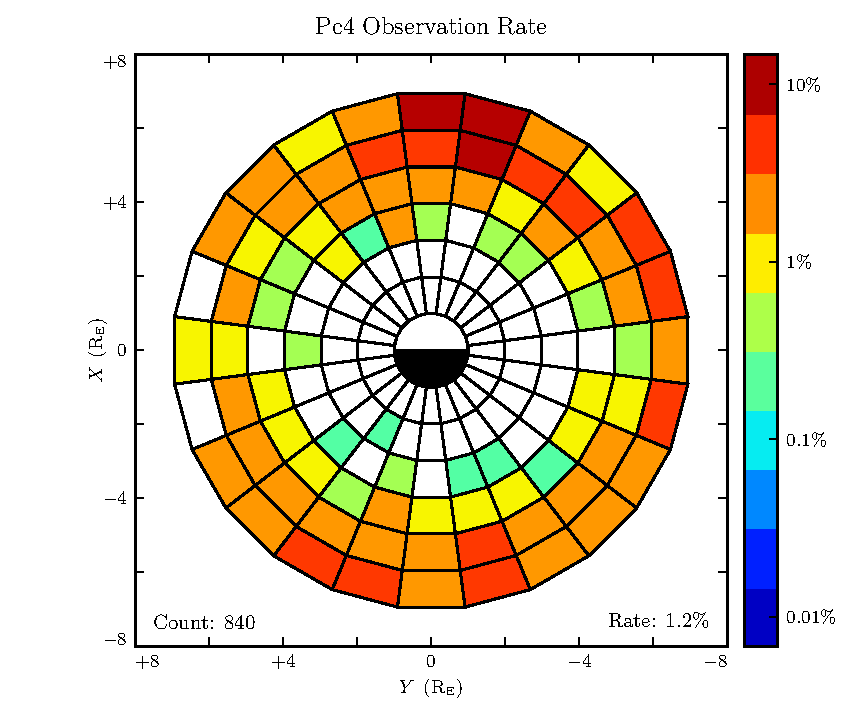
\includegraphics[width=\textwidth]{figures/rate_all_sharp.pdf}
    \caption[Observation Rate of Pc4 Events]{
      The above figure shows the spatial distribution of all 840 observed Pc4 events. Counts are normalized by the amount of usable data in each bin. The value in the bottom-right corner is the mean of the rate in each bin; it's an estimate of how often Pc4 events would be observed if the sampling were distributed uniformly in space. Events where the poloidal and toroidal channel trigger simultaneously (\about\SI{10}{\percent} of cases) are counted as only a single event. Bins shown in white contain zero events. 
    }
    \label{fig_rate_all_sharp}
\end{figure}

Consistent with previous work, Pc4 events are rarely observed at $L < 4$. Nearly \SI{30}{\percent} of the usable data shown in \cref{fig_pos_all_sharp} is located inside $L = 4$, yet that data accounts for only 18 of the 840 events. 

\todo{Dai thinks that Pc4 pulsations are common inside the plasmasphere. He uses the plasma number density gradient to estimate the plasmapause location. We use Scott's method, which is a cutoff of \SI{100}{\percc}. We find basically no events inside the plasmapause --- only 43 out of 840. }

In \cref{fig_mode_all_sharp}, events are partitioned by parity and polarization, yielding 141 odd poloidal events, 237 even poloidal events, 457 odd toroidal events, and 87 even toroidal events --- a total of 922 events. The total is greater than 840 because in \about\SI{10}{\percent} of events, the poloidal and toroidal channels trigger independently. Such cases count as only a single event in \cref{fig_rate_all_sharp}, but the toroidal and poloidal events are both shown in \cref{fig_mode_all_sharp}. 

\todo{Even poloidal events and even toroidal events are distributed similarly, which is good to see, since even poloidal events give rise to even toroidal events. The relationship is less clear for odd events, though odd poloidal modes and odd toroidal modes are both least common at dusk. }

\todo{Odd toroidal events are by far the most commonly observed. Oddly, even poloidal events are the least common. }

\todo{Even modes are less likely to be observed on the ground? \cite{takahashi_1992} }

\begin{figure}[!htb]
    \centering
    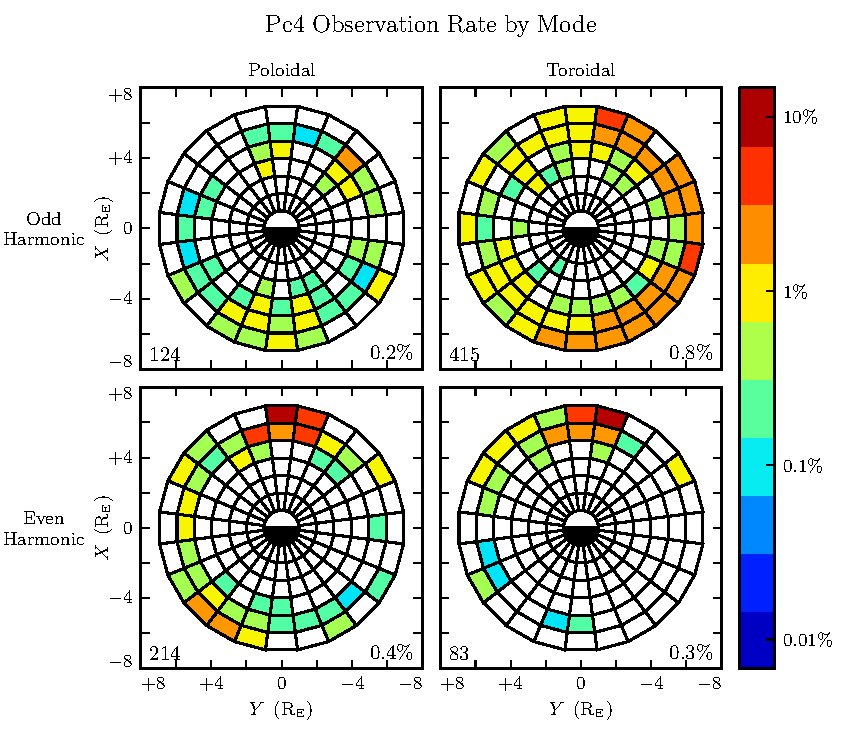
\includegraphics[width=\textwidth]{figures/mode_all_sharp.pdf}
    \caption[Observation Rate of Pc4 Events by Mode]{
      The above figure shows the spatial distribution for the same 840 events shown in \cref{fig_rate_all_sharp}, partitioned by polarization and parity. The selection criteria described in \cref{sec_selection} ensure that both properties are known for all events. Event counts are normalized by the time spent by the amount of usable data in each bin. Event counts do not sum to 840 because some events trigger on both the poloidal channel and the toroidal channel. Bins shown in white contain zero events. 
    }
    \label{fig_mode_all_sharp}
\end{figure}

% -----------------------------------------------------------------------------
% -----------------------------------------------------------------------------
% -----------------------------------------------------------------------------
\section{Rate of Pc4 Events by Amplitude}
  \label{sec_amp}


\begin{figure}[!htb]
    \centering
    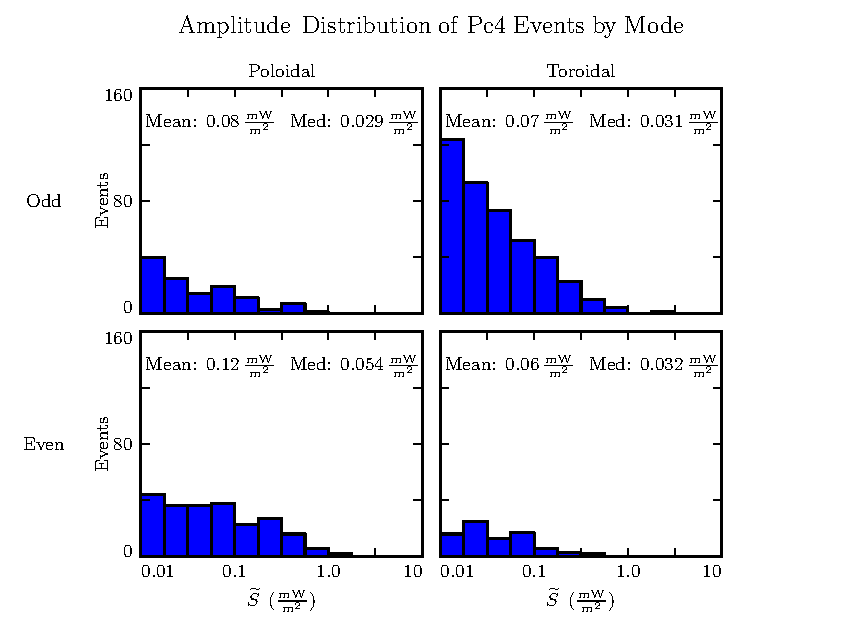
\includegraphics[width=\textwidth]{figures/amp.pdf}
    \caption[TEST FIGURE]{
      \todo{$\cdots$}
    }
    \label{fig_amp}
\end{figure}


\begin{figure}[!htb]
    \centering
    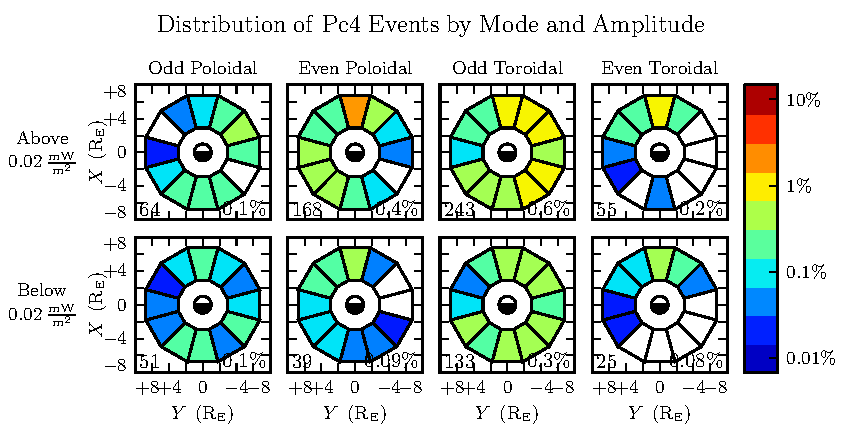
\includegraphics[width=\textwidth]{figures/mode_amp.pdf}
    \caption[TEST FIGURE]{
      \todo{$\cdots$}
    }
    \label{fig_mode_amp}
\end{figure}


% -----------------------------------------------------------------------------
% -----------------------------------------------------------------------------
% -----------------------------------------------------------------------------
\section{Rate of Pc4 Events by Frequency}
  \label{sec_f}



\begin{figure}[!htb]
    \centering
    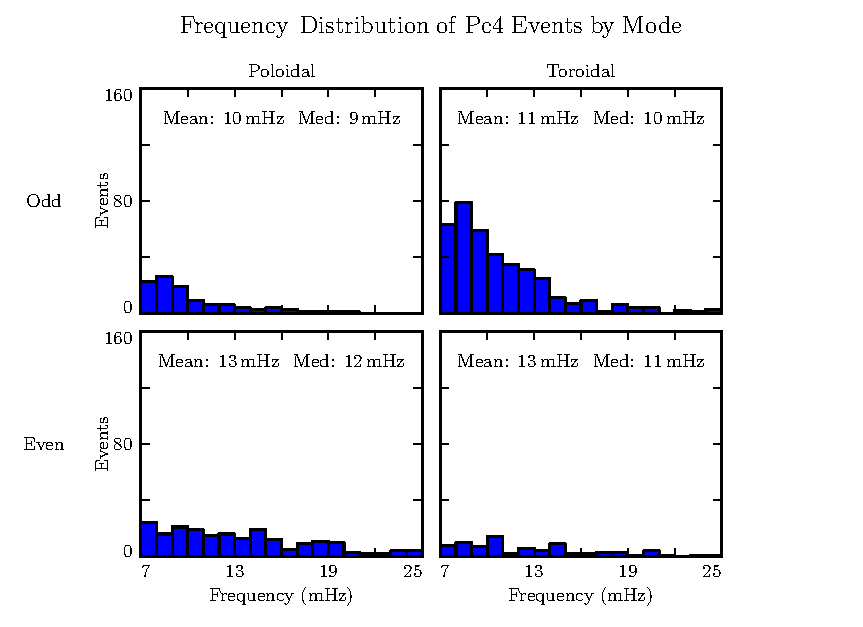
\includegraphics[width=\textwidth]{figures/f.pdf}
    \caption[TEST FIGURE]{
      \todo{$\cdots$}
    }
    \label{fig_f}
\end{figure}


\begin{figure}[!htb]
    \centering
    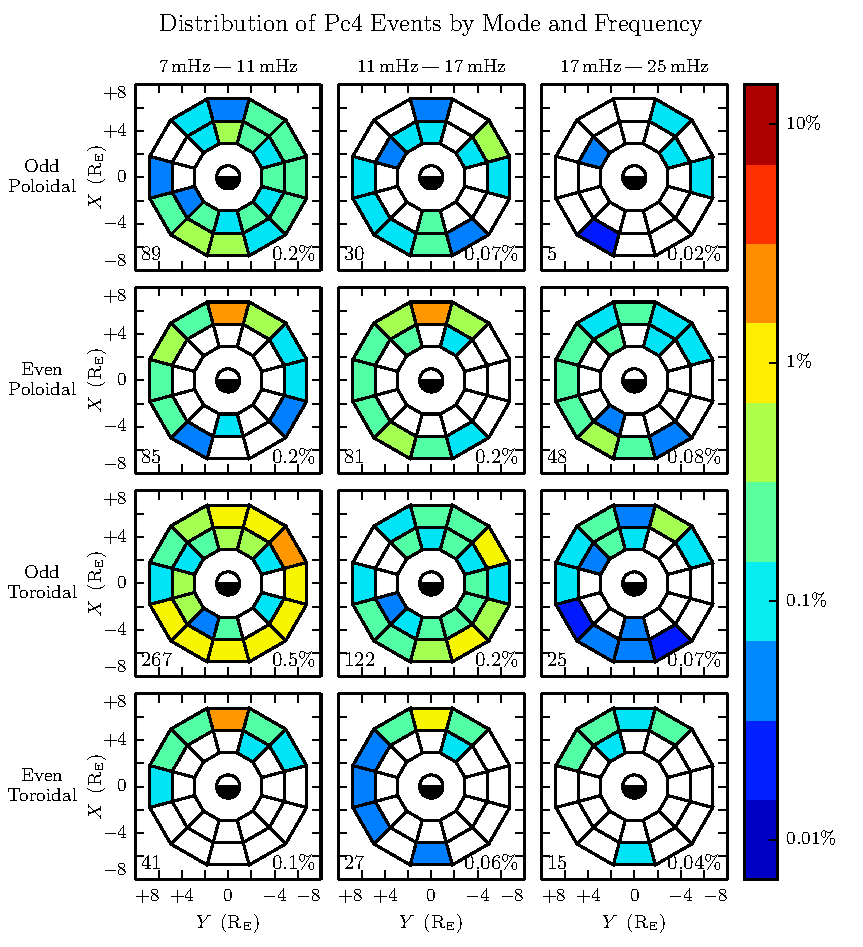
\includegraphics[width=\textwidth]{figures/mode_f.pdf}
    \caption[TEST FIGURE]{
      \todo{$\cdots$}
    }
    \label{fig_mode_f}
\end{figure}


% -----------------------------------------------------------------------------
% -----------------------------------------------------------------------------
% -----------------------------------------------------------------------------
\section{Rate of Pc4 Events by Phase}
  \label{sec_phase}




\begin{figure}[!htb]
    \centering
    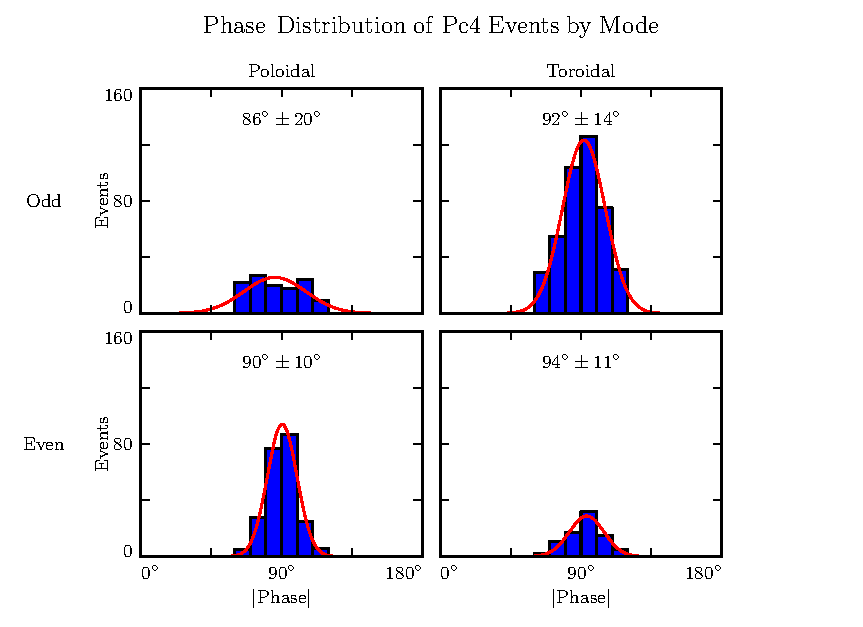
\includegraphics[width=\textwidth]{figures/phase.pdf}
    \caption[TEST FIGURE]{
      \todo{$\cdots$}
    }
    \label{fig_phase}
\end{figure}


\begin{figure}[!htb]
    \centering
    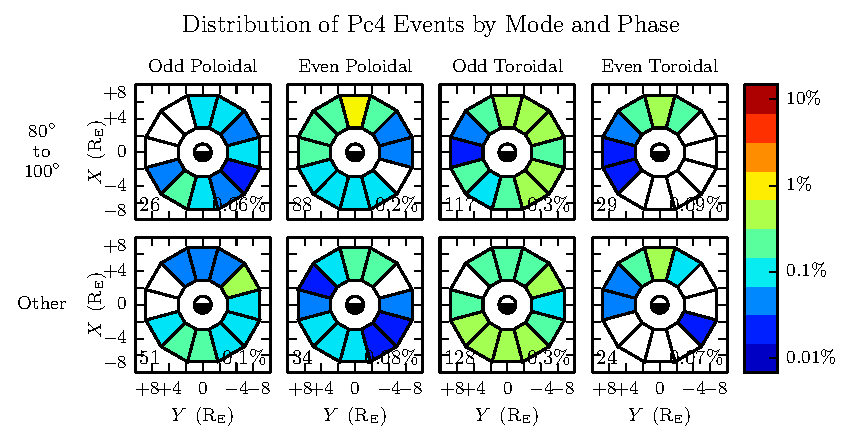
\includegraphics[width=\textwidth]{figures/mode_phase.pdf}
    \caption[TEST FIGURE]{
      \todo{$\cdots$}
    }
    \label{fig_mode_phase}
\end{figure}


% -----------------------------------------------------------------------------
% -----------------------------------------------------------------------------
% -----------------------------------------------------------------------------
\section{Rate of Pc4 Events by Spectral Width}
  \label{sec_fwhm}



\begin{figure}[!htb]
    \centering
    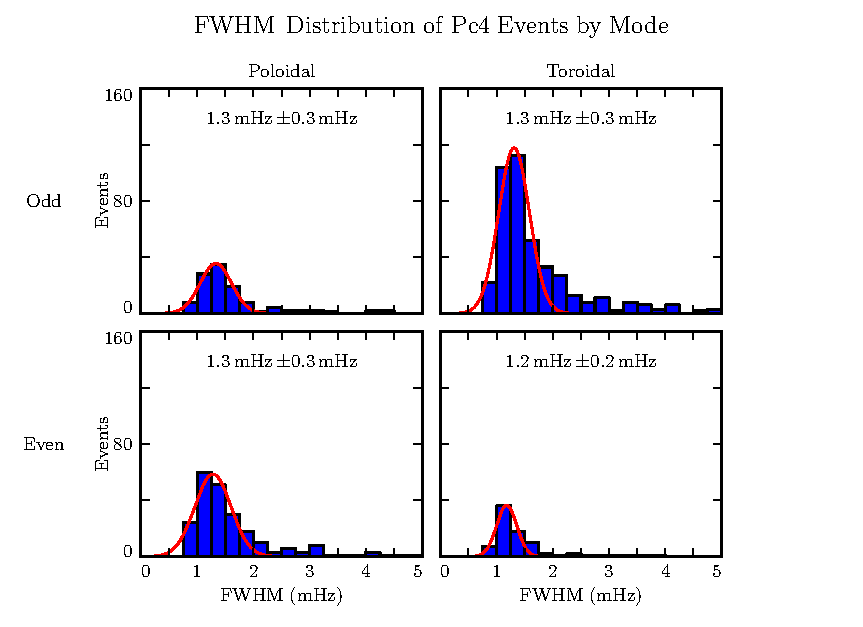
\includegraphics[width=\textwidth]{figures/fwhm.pdf}
    \caption[TEST FIGURE]{
      \todo{$\cdots$}
    }
    \label{fig_fwhm}
\end{figure}


\begin{figure}[!htb]
    \centering
    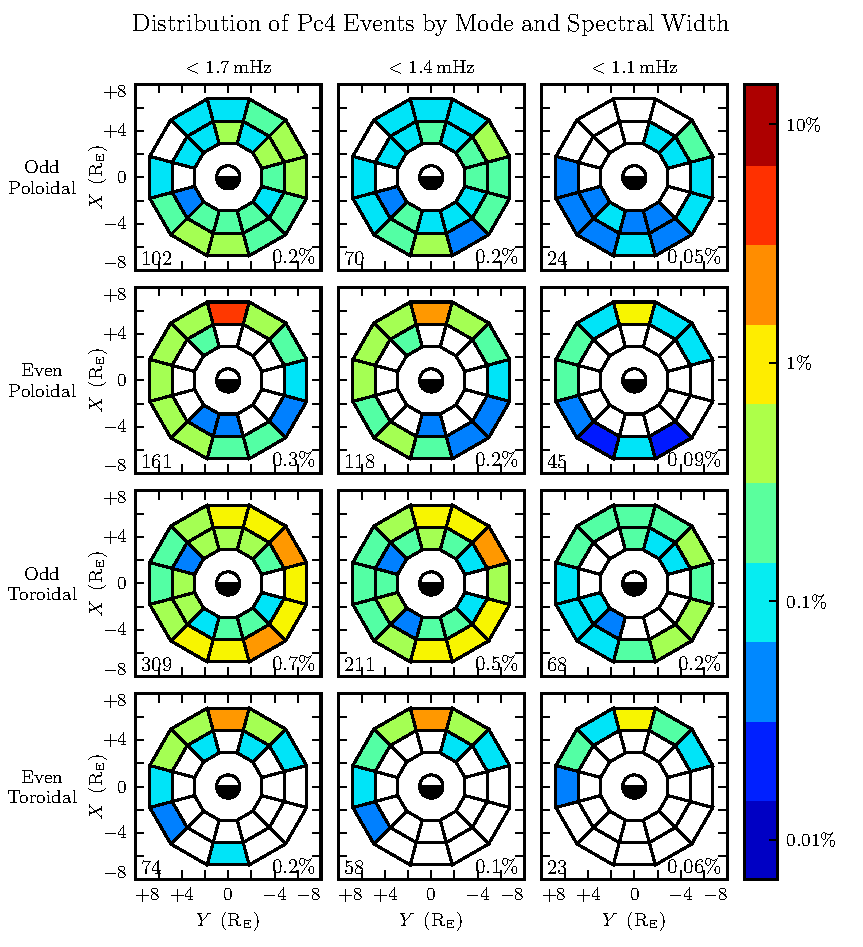
\includegraphics[width=\textwidth]{figures/mode_fwhm.pdf}
    \caption[TEST FIGURE]{
      \todo{$\cdots$}
    }
    \label{fig_mode_fwhm}
\end{figure}




% -----------------------------------------------------------------------------
% -----------------------------------------------------------------------------
% -----------------------------------------------------------------------------
%\section{Poloidal Pc4 Events by Compressional Coupling}

%\todo{Low-\azm poloidal Pc4 events are coupled to the compressional mode, while high-\azm ones are not. }

%\todo{The value of $\dft{B_z}/\dft{B_x} = 0.2$ comes from Dai\cite{dai_2015}. Can we match this up to an \azm value? Sounds like a job for Tuna! }

%\begin{figure}[!htb]
%    \centering
%    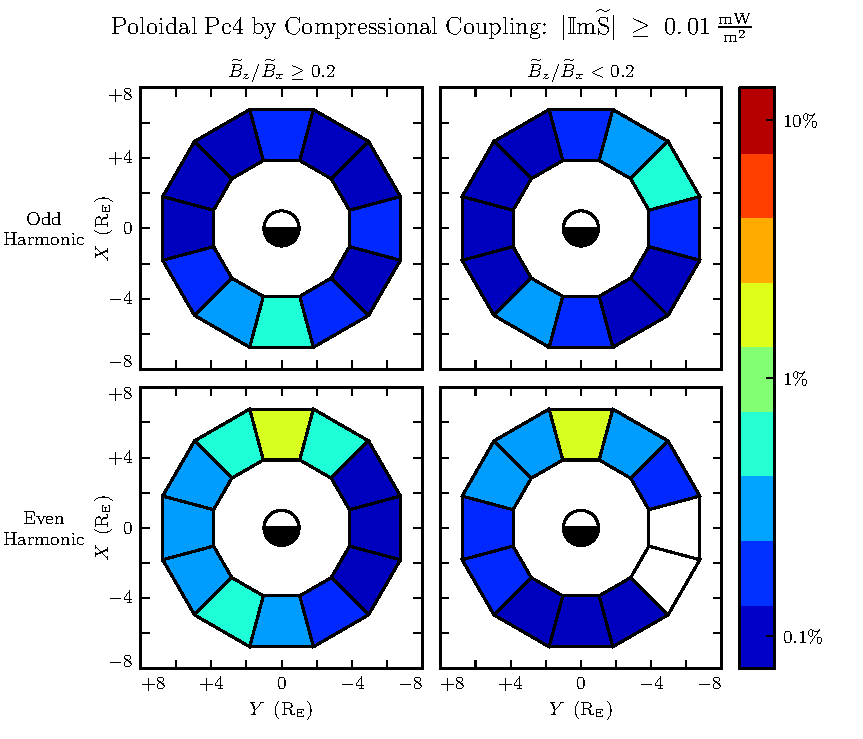
\includegraphics[width=\textwidth]{figures/azm_rate_all.pdf}
%    \caption[Poloidal Pc4 Rate by Compressional Coupling]{
%      \todo{Odd poloidal Pc4 events have a peak pre-noon and another peak near midnight. The pre-noon peak seems to be composed of high-\azm events, and the midnight peak seems to be low-\azm events. Low-\azm even poloidal events are spread broadly across the dusk side, while high-\azm even events are peaked strongly on the dayside --- consistent with Dai's results\cite{dai_2015}. }
%    }
%    \label{fig_azm_rate_all}
%\end{figure}


% -----------------------------------------------------------------------------
% -----------------------------------------------------------------------------
% -----------------------------------------------------------------------------
\section{Discussion}

\todo{$\cdots$}



%\todo{Collections of events at a single ground observatory (near \SI{66}{\degree}) over significant periods of time: }

%Brekke\cite{brekke_1987} looked at 523 giant pulsation events recorded at Troms{\o}, Norway, from 1929 to 1985. This spanned several solar cycles. 

%Rolf\cite{rolf_1931} collected 28 events between 1921 and 1930 at Abisko. 

%Sucksdorf\cite{sucksdorff_1939} got 150 events between 1914 and 1938 in Sodankyl{\"a}. 

%Harang\cite{harang_1941}. 97 events from 1929 to 1941. Also Troms{\o}. Note that this may have been limited by the war! 

%This comes out to something like ... events over ... years. That's about ... giant pulsations per year, observed on the ground. 

%\todo{Collections of events at an array of ground observatories: }

%Chisham and Orr\cite{chisham_1991} found 34 events from 1984 to 1987 using the EISCAT magnetometer array in scandanavia. About \SI{5}{\degree} in MLT, decent coverage from \SIrange{63}{67}{\degree} mlat. This coincides with a solar minimum. 

%Motoba, in 2015, recorded 105 giant pulsation events. The observations were carried out by a number of ground magnetometers spanning $\sim \SI{90}{\degree}$ in local time and ranging roughly \SIrange{60}{70}{\degree} magnetic latitude\cite{motoba_2015}. This was mostly during a period of low solar activity, so we expect a high count. 

%\todo{Estimate of the size of an event's footprint:}

%Velkamp\cite{veldkamp_1960} looked at a single large event and showed that, at best, it was visible over a span of \SI{5}{\degree} in magnetic latitude. 

%This is seemingly consistent with the 29 February 2012 event discussed in detail by Motoba\cite{motoba_2015} --- Motoba shows some data, but doesn't discuss this aspect in detail. 

%Takahashi\cite{takahashi_2011} computes a FWHM of about 1 in L, or \SI{2}{\degree} magnetic latitude. 

%\todo{Tying that in to RBSP observations? }

%Note that it's a bit tricky to compare ground observations to in situ observations. Large-\azm events won't make it through the ionosphere. 

%There should be no bias with respect to MLT between a ground magnetometer and RBSP. Dai's analysis was specifically chosen to take advantage of the fact that RBSP's orbit had precessed all the way around the Earth. No preferred direction. And mlat shouldn't cause issues... these are FLRs, after all. 

%How strong does an event need to be on the ground, or in the sky, to count as a giant pulsation? Motoba 2015\cite{motoba_2015} has an event which tops out on the order of \SI{10}{\nT} on the ground. It's more like \SI{5}{\mV/\m} in situ. Takahashi\cite{takahashi_2011} has similar values. 

%If peak Pg observations are at $\SI{66}{\degree}$ mlat, that corresponds to $L = 6$. Then let's suppose that peak Pg viewing is $\SI{5}{\degree}$ wide --- estimating from the work of Velkamp and Motoba. That means RBSP should see lots of Pgs when it's between $L = 5.2$ andn $L = 7.1$. Well, \SI{7.1}{\RE} is outside its apogee, but the probes spend a fair amount of time outside $L = 5.2$, since they are moving pretty slowly at that point. 

%Giant pulsations have been shown to be more numerous in times of low solar activity. That was the whole point of Brekke's seminal 1987 paper, and it's consistent with what we show in \cref{ch_results}. The RBSP observations occur during peak solar times, though it's an anemic solar peak\cite{pesnell_2016}. 

%\todo{How much time does RBSP spend outside of $L = 5.2$ (for a range of \SI{5}{\degree})? How about $L = 5.6$ to $L = 6.5$ (for FWHM of \SI{2}{\degree}? }

%Each RBSP probe spends about \SI{30}{\percent} of its orbit between $L = 5.6$ and $L = 6.5$. 

%RBSP-A and RBSP-B count as two observers. In one $\sim 5$ cases out of hundreds do they simultaneously observe a poloidal Pc4 event (although, most notably for the 2012 event which \cite{dai_2013} considers in detail), both probes do fly through the same apparent event several hours apart from one another. 

%The duration of Dai's survey is October 2012 to June 2014. Scaled by 2 probes, each of which is present in the peak Pg lshells 30\% of the time, that comes out to almost exactly one year. 

%\todo{How many fundamental mode poloidal events do we see? How many could pass for giant pulsations? How many should we expect to see? }

%\todo{How weird is it for a fundamental mode poloidal Pc4 to be monochromatic? }

%\todo{How weird is it for a fundamental mode poloidal Pc4 to be stronger than \SI{5}{\mV/\m} at the equator? }






